%\documentclass{beamer}
\documentclass[handout]{beamer}
\usetheme{default}
\usepackage[spanish]{babel}
\usepackage[utf8]{inputenc}
\usepackage{amsmath}
\usepackage{tipx}
\usepackage{color}
\usepackage{hyperref}

\usepackage{pgfpages}
\pgfpagesuselayout{2 on 1}[a4paper,border shrink=5mm]

% items enclosed in square brackets are optional; explanation below
\title[Comunicación]{¿Qué son las lenguas?}
%\subtitle[Signo]{El Signo}
\author[V. Peinado]{Víctor Peinado}
\institute[UCM]{
  \texttt{v.peinado@filol.ucm.es}\\[1ex]
  
  Grado de Logopedia, Universidad Complutense de Madrid\\[1ex]
}

\date[Noviembre 2010]{24 de octubre - 14 de noviembre de 2011}

\begin{document}

\let\ipa\textipa
\let\it\textit

%--- the titlepage frame -------------------------%
\begin{frame}[plain]
  \titlepage
\end{frame}

%--- the presentation begin here -----------------%

\begin{frame}{}
\begin{center}
\LARGE ¿Cuántas lenguas hay?
\end{center}
\end{frame}


\begin{frame}{¿Cuántas lenguas hay?}

\begin{itemize}
	\item Es una de las primeras preguntas que siempre hacen los no lingüistas.
	\item Como nuestra lengua es algo que sentimos tan propio, las lenguas extranjeras siempre nos han llamado la atención.
	\item El mito de la torre de Babel y otros similares han tratado, desde la antigüedad de explicar por qué hay lenguas distintas.
	\item Los griegos antiguos llamaban \textit{bárbaros} a los extranjeros que no sabían expresarse correctamente en su lengua: en realidad, $\beta\alpha\rho\beta\alpha\rho o\varsigma$ simplemente significa «tartamudo».
	\item Hay chistes de todo tipo sobre lo raro o divertido que hablan los extranjeros.
\end{itemize}

\end{frame}


\begin{frame}{¿Cuántas lenguas hay?}

\begin{itemize}
	\item Por si esto fuera poco, dentro de cada lengua existe mucha diversidad. A menudo se dice que determinadas personas «hablan mal», «se comen letras», «tienen acento» o «no se les entiende».
	\item Todo ello conduce siempre al mismo punto de partida $\rightarrow$ la única lengua de verdad es la mía.
	\item Suele existir una identificación entre grupo étnico y lengua. Esta identificación, como veremos más adelante, puede ser correcta, aunque no siempre lo es. Hay que ser cuidadosos.
	\item Aprender una lengua extranjera es una tarea ardua y difícil: es casi imposible dejar de hablar con acento extranjero.
	\item La diversidad lingüística es un misterio. Saber cuántas lenguas hay en el mundo no es un pregunta tonta.
	\item Lo malo no es la pregunta, sino la respuesta.
\end{itemize}

\end{frame}

\begin{frame}{¿Cuántas lenguas hay?}
\begin{itemize}

	\item No sabemos cuántas lenguas hay y es imposible saberlo.
	\item Habitualmente se habla de entre 3.000 y 6.000 lenguas. 
	\item Los recuentos más amplios (véase el catálogo de \href{http://www.ethnologue.com}{Ethnologue}) llegan casi a 7.000, pero incluyen lenguas extintas.
	\item Estos números no nos dicen gran cosa. Nos dicen que hay muchas lenguas, pero no tantas como podría haber. 
	\item Somos 7.000.000.000 personas en el mundo, salimos a casi 1 millón de habitantes por lengua.
	\item Sin embargo, el reparto es desigual: hay lenguas (unas pocas) con muchos millones de hablantes y muchas lenguas (la gran mayoría) con pocos hablantes, algunas incluso con menos de un centenar.
\end{itemize}

\end{frame}

\begin{frame}{¿Cuántas lenguas hay?}
\begin{itemize}
	\item Hay 194 estados reconocidos internacionalmente: nos toca a unas 33 lenguas por país.
	\item Pero el reparto geográfico también es muy desigual y no entiende de fronteras.
		\begin{itemize}
			\item América tiene el 15\% de las lenguas.
			\item África tiene el 30\% de las lenguas.
			\item Asia tiene el 32\% de las lenguas.
			\item Australia y los países del Pacífico poseen el 19\% de las lenguas.
			\item El 4\% restante se reparte entre Europa y Oriente Medio.
		\end{itemize}
	\item El reparto de lenguas por países es todavía más curiosa:
	\begin{itemize}
		\item España, con 46M habitantes, tiene 4 lenguas oficiales.
		\item Camerún, con solo 17M habitantes y una extensión menor que España, tiene 286 lenguas. 
		\item En toda Europa hay 225 lenguas.
		\item En India hay 360 lenguas, Nigeria tiene 450 y Papúa Nueva Guinea tiene ¡850 lenguas distintas!
	\end{itemize}
\end{itemize}
\end{frame}

\begin{frame}{Reparto geográfico de las lenguas}

Cada punto representa el centro geográfico aproximado de una lengua.

\begin{center} 
  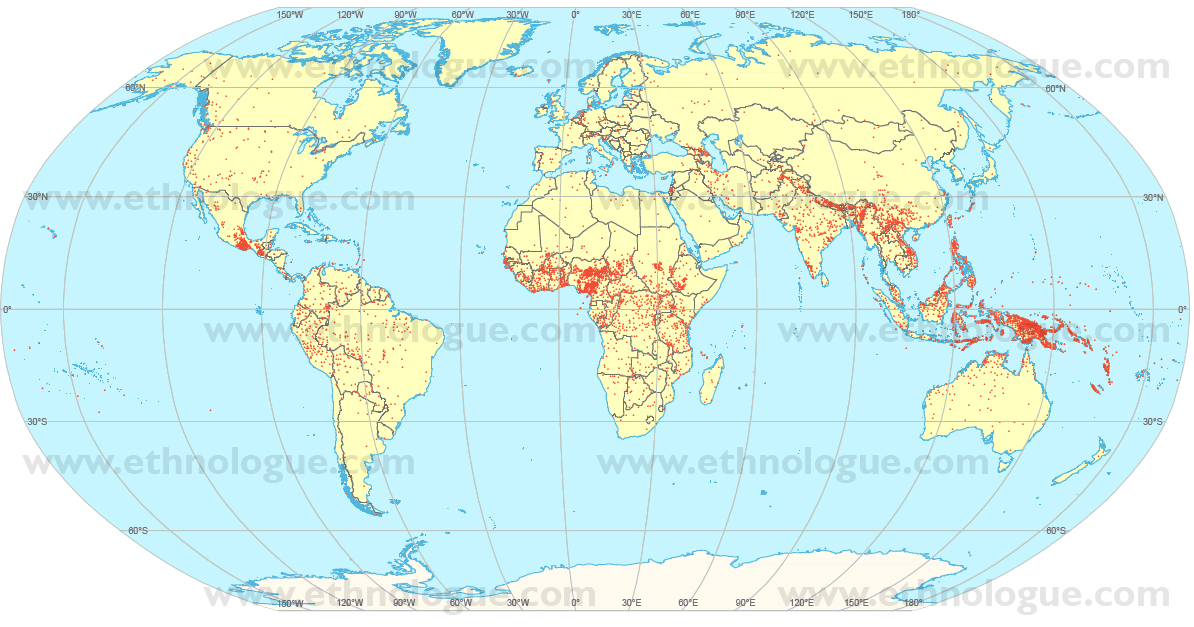
\includegraphics[scale=0.35]{img/wrld_eth.jpg} 
\end{center}
\end{frame}


\begin{frame}{¿Cuántas lenguas hay?}
\begin{itemize}
	\item Si atendemos al número de hablantes, solo hay unas 600 lenguas que tengan más de 100.000 hablantes
	\item 100.000 hablantes es la cifra que se suele mencionar como el umbral mínimo a partir del cual se considera que una lengua no está en peligro de desaparición a medio plazo.
	\item Y solo 250 lenguas tienen más de 1M hablantes, son las grandes lenguas del mundo: 
	\begin{itemize}
		\item chino mandarín, español, inglés, hindi, bengalí, portugués, ruso, árabe, japonés y francés son las 10 primeras por número de hablantes nativos.
	\end{itemize}
	\item Véase la \href{http://es.wikipedia.org/wiki/Anexo:Lenguas_por_n\%C3\%BAmero_de_hablantes}{tabla de lenguas por número de hablantes}
\end{itemize}
\end{frame}

\begin{frame}{¿Cuántas lenguas hay?}
\begin{enumerate}
	\item ¿Qué es una lengua? (y un dialecto, y todo eso)
	\item ¿Por qué hay tantas? (o tan pocas)
	\item ¿De dónde han salido? ¿Cómo se relacionan unas con otras? (si es que se relacionan)
	\item ¿Qué sucede con las lenguas al pasar el tiempo? ¿Desaparecen?
	\item ¿Hay más lenguas ahora que en épocas anteriores o menos?
	\item ¿Hay lenguas mejores o peores, más o menos primitivas, más o menos perfectas, más o menos puras?
	\item ¿Cómo cambian las lenguas?
\end{enumerate}
\end{frame}



\begin{frame}{¿Qué es una lengua?}

\begin{itemize}
	\item Las lenguas que podemos observar varían enormemente.
	\item El español y el chino son muy distintas entre sí. 
	\item El español y el inglés son distintas también, pero las diferencias son menores.
	\item Aún menor es la diferencia que percibimos con el italiano o con el gallego. 
	\item Mi primo de Ciudad Real y mi suegra de Sevilla no hablan igual que yo, pero las diferencias, aunque existen, son mínimas.
	\item No hay dos personas que hablan igual. Una misma persona habla de manera diferente a lo largo de su vida, incluso en distintos momentos a lo largo de un mismo día.
	\item No hablamos igual que escribimos.
\end{itemize}
\end{frame}

\begin{frame}{¿Qué es una lengua?}

\begin{itemize}
	\item Si no sabemos definir de manera clara qué es una lengua difícilmente podremos contarlas. O los distintos intentos de catalogar las lenguas del mundo darán números dispares.
	\item La dificultad para enumerar las lenguas del mundo radica en que \textcolor{blue}{existe un continuo, una diferenciación gradual}, entre las distintas variedades de lengua que utiliza una misma persona a lo largo de un día (p. ej., cuando habla entre amigos y cuando declara ante un juez) y las diferencias radicales que existen entre el chino y el español.
	\item Sin embargo, por muy diferentes que sean dos lenguas, algo de común permanece. De manera que nunca confundimos dos lenguas humanas con cualquier mecanismo de comunicación animal.
	\item Las lenguas humanas, a pesar de sus diferencias, son básicamente distintas variantes de una misma cosa. Si las comparamos con el lenguaje de las abejas o los bonobos, las lenguas humanas se parecen bastante entre sí.
\end{itemize}
\end{frame}

\begin{frame}{¿Cuántas lenguas hay en España?}
\begin{itemize}
	\item En España hay cuatro lenguas oficiales: castellano, catalán, gallego y vasco.
	\item Sin embargo, \href{http://www.ethnologue.com/show_country.asp?name=ES}{Ethnologue enumera hasta 14 lenguas para España}.
	\pause
	\begin{itemize}
		\item castellano, catalán/valenciano/balear, gallego, vasco, aragonés, bable, caló, extremeño, chapurreau, gascón/aranés, y tres lenguas de señas (española, catalana y valenciana). 
	\end{itemize}
	\item ¿En qué podemos basarnos para contar las lenguas? ¿En la capacidad para entendernos?
\end{itemize}

\end{frame}

\begin{frame}{¿Cuántas lenguas hay en España?}
\begin{itemize}
	\item Utilizar el criterio de la \textcolor{blue}{inteligibilidad} no siempre es sencillo.
	\item Los castellano-hablantes, por regla general, podemos entender sin mucha dificultad el gallego normativo, no así el gallego hablado en determinadas zonas rurales.
	\item Entendemos con menor frecuencia el catalán. 
	\item Nunca entendemos el vasco.
	\item A veces es más sencillo entender a un valenciano (hablando otra lengua) que a un gaditano (oficialmente, habla nuestra misma lengua).
	\item En la \textcolor{blue}{capacidad de comprensión también existe un continuo}.
	\item No hay duda de que los castellano-hablantes no comprenden a los hablantes de inglés, chino o !kung $\rightarrow$ son lenguas distintas.
\end{itemize}
\end{frame}

\begin{frame}{Lenguas de los países escandinavos}
\begin{itemize}
	\item Si salimos de España, sucede lo mismo: ¿Cuántas lenguas hay en Escandinavia? 
\end{itemize}
	\begin{center} 
	  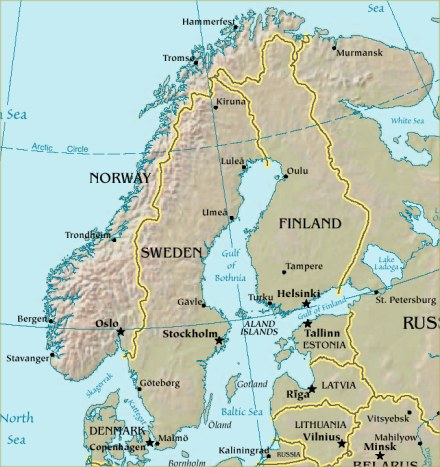
\includegraphics[scale=1]{img/scandinavia.jpg} 
	\end{center}
\end{frame}

\begin{frame}{Lenguas de los países escandinavos}
\begin{itemize}
	\item Simplificando un poco, oficialmente, hay cuatro lenguas: danés, noruego, sueco y finés.
	\item El finés es de la famila ugro-fínica y resulta incomprensible para el resto. Nos olvidamos de él por el momento.
	\item Las otras tres lenguas son de la familia germánica: genéticamente están emparentadas y por razones históricas y culturales, han tenido contacto continuo durante siglos.
	\item El danés es difícil de comprender por el resto, salvo por los suecos del sur, que lo entiende bastante bien. 
	\item Suecos y noruegos, por lo general, se entienden aunque hablan oficialmente lenguas distintas. 
	\item Algunos noruegos del este comprenden mejor a los suecos del oeste que a algunas variedades del noruego.
	\item Hay un \textcolor{blue}{continuo} en la inteligibilidad de estas lenguas.
\end{itemize}
\end{frame}

\begin{frame}{Lenguas de la ex-Yugoslavia}
\begin{itemize}
	\item ¿Cuál es la situación lingüística de los países de la ex-Yugoslavia? 
\end{itemize}
	\begin{center} 
	  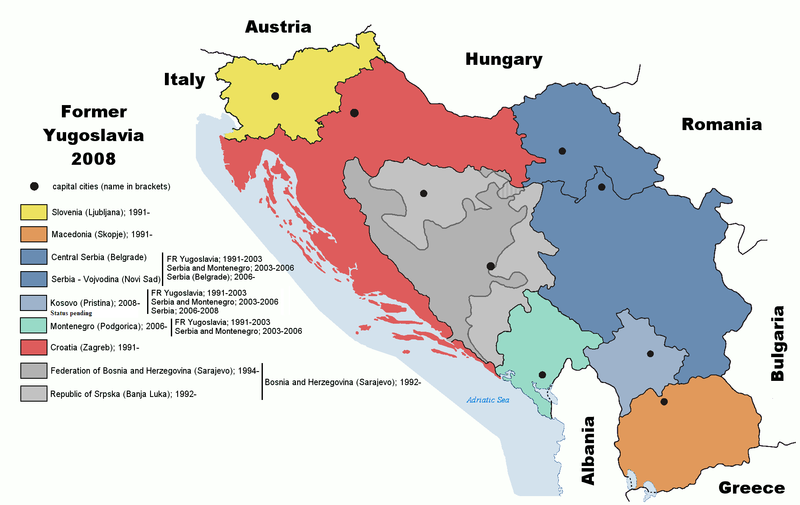
\includegraphics[scale=0.35]{img/yugoslavia.png} 
	\end{center}
\end{frame}

\begin{frame}{Lenguas de la ex-Yugoslavia}

\begin{itemize}
	\item Antes de la guerra se hablaban oficialmente tres lenguas:
	\begin{itemize}
		\item esloveno en el noroeste.
		\item macedonio en el sureste.
		\item serbocroata en el resto.
	\end{itemize}

	\item El serbo-croata estaba formado por dos ¿variantes/dialectos? mutuamente inteligibles, aunque utilizaban alfabetos diferentes:

	\begin{itemize}
		\item los croatas utilizaban el alfabeto latino.
		\item los serbios utilizaban el alfabeto cirílico.
	\end{itemize}

	\item Tras la guerra, se habla no de dos lenguas, sino de tres: 
	\begin{itemize}
		\item croata
		\item serbio
		\item bosnio
	\end{itemize}
	\item ¿Acaso han nacido de un día para otro una, dos o tres lenguas nuevas? Lingüísticamente, tras la guerra nada ha cambiado. 
	\item La definición de \textcolor{blue}{lenguas distintas} casi nunca es una cuestión lingüística. 
	\end{itemize}
\end{frame}

\begin{frame}{Situación del ebónico}
\begin{itemize}
	\item A finales de los 1990s, hubo mucha polémica en EEUU acerca de si el ebónico era un dialecto del inglés o una lengua diferente.
	\item Ebónico es la denominación, políticamente correcta, para llamar al \it{black english} o \it{African American Vernacular English}: la variante del inglés que utilizan mayoritariamente los negros de EEUU.
	\item Las autoridades de la ciudad de Oakland, CA razonaron:
	\begin{itemize}
		\item los niños negros tienen peores resultados en la escuela porque no hablan inglés estándar, sino ebónico.
		\item en consecuencia, los niños negros no entienden a sus profesores y tiene dificultad para expresarse en inglés estándar.
		\item algo parecido les pasa a los niños latinos, chinos, indios, etc., pero a estos se les enseña inglés porque hablan una lengua distinta.
		\item Hay que tratar a los niños negros como si fuesen hablantes de lengua extranjera y formar a los profesores en ebónico.
	\end{itemize}
\end{itemize}
\end{frame}

\begin{frame}{}
\begin{center}
\LARGE Lenguas, dialectos, hablas, jergas
\end{center}
\end{frame}


\begin{frame}{Lenguas, dialectos, hablas, jergas}
\begin{itemize}
	\item Estos términos para los lingüistas no tienen ningún tipo de connotación. Se utilizan de manera neutra.
	\item Sin embargo, cotidianamente palabras como dialecto y jerga se suele utilizar de manera peyorativa.
	\item Socialmente están muy marcados y a menudo se exige a los lingüistas que expliquen las diferencias entre ellos.
	\item Es habitual encontrar opiniones en la prensa que defienden cosas como las siguientes:
	\begin{itemize}
		\item Las lenguas son superiores, tienen tradición escrita, merecedoras de una cultura rica y son símbolo identitario de un país.
		\item Los dialectos son cosas menores, patrimonio cultural, sí, pero de estar en casa. Cosa de canciones populares y bailes regionales.
	\end{itemize}
\end{itemize}
\end{frame}

\begin{frame}{Lenguas, dialectos, hablas, jergas}
\begin{itemize}
	\item Algunas escuelas lingüísticas han intentado eliminar este sentido peyorativo proponiendo otros términos.
	\item las \textcolor{blue}{variantes diatópicas} son las formas particulares que adopta una lengua en las diferentes regiones o áreas geográficas.
	\item las \textcolor{blue}{variantes diastráticas} son las diferencias sociales entre clases y estratos sociales, o entre grupos profefesionales.
	\item los \textcolor{blue}{lenguajes especiales} son las jergas, las formas de una lengua que adoptan grupos especiales.	
	\item Estas denominaciones, frecuentes en sociolingüística, no se utilizan en la vida cotidiana.
\end{itemize}
\end{frame}

\begin{frame}{Lenguaje}
\begin{itemize}
	\item Utilizaremos este término para lo que es común a todas las lenguas humanas, incluso lo podemos ampliar a las formas de comunicación animal.
	\item Fundamentalmente, se trata de la capacidad que poseemos los seres humanos para hacer ciertas cosas por medio de señales sonoras o visuales.
\end{itemize}
\end{frame}


\begin{frame}{Lengua}
\begin{itemize}
	\item Sigue siendo complicado definir qué es una lengua.
	\item No es posible dar una definición puramente lingüística.
	\item No todos los hispanohablantes hablamos igual, aunque a la hora de escribir nuestro estilo sí se parece más.
	\item Todos los hispanohablantes somos conscientes de una forma más o menos vaga de que compartimos algo: hablamos la misma lengua.
	\item Una lengua es un ente abstracto, un ideal al que los hablantes, supuestamente, aspiran llegar.
	\item Una lengua es un consenso social.
	\item Véase el vídeo \href{http://www.youtube.com/watch?v=sBiM3ELPjXs}{Moreno Cabrera: el español estándar}.

\end{itemize}

\end{frame}


\begin{frame}{Lengua estándar o norma culta}
\begin{itemize}
	\item Normalmente, cuando pensamos en lengua nos referimos (casi siempre sin saberlo) a la \textcolor{blue}{lengua estándar}.
	\item La lengua estándar es lo que se aprende en las escuelas y se enseña a los extranjeros.
	\item Normalmente, la mayoría de los textos están escritos en estándar.
	\item Es la forma de la lengua que se utiliza para dar conferencias y clases, en debates políticos, etc.
	\item El castellano, el catalán, el inglés, el alemán\ldots todas las lenguas occidentales tienen una variante estándar que se utiliza en estos contexto anteriores.
	\item Hay bastante gente que, en el ámbito privado, puede usar otras formas de «lengua española»: p. ej., hay gente que en casa habla el «granadino cerrado», es decir, el dialecto o variante diatópica de Granada.
	\item En ello no hay nada de malo o incorrecto.
\end{itemize}
\end{frame}

\begin{frame}{Lengua estándar}
\begin{itemize}
	\item El estándar nos permite dirigirnos a cualquier hispanohablante o a cualquier persona que haya aprendido español sin problemas graves de comunicación. 	
	\item El estándar no es la consagración del hablar bien.
	\item El estándar es simplemente un acuerdo social, más o menos tácito, que permite entenderse perfectamente a un conjunto de personas. 
	\item El vocabulario estándar no es de ningún sitio porque es de todas partes a la vez.
	\item Si una palabra que utilizamos cotidianamente no está en el estándar, significa que no la entienden todos los hispanohablantes.
	\item Que una palabra figure o no en el diccionario académico no significa nada. No es mejor ni peor. 
	\item El estándar es una norma social. Y como cualquier norma de conducta social, cambia con el paso del tiempo.
\end{itemize}
\end{frame}

\begin{frame}{Hablar bien o hablar mal}
\begin{itemize}
	\item Es habitual escuchar cosas como «los leistas hablan mal», «decir treceavo para indicar el ordinal es incorrecto», «la expresión ``las tareas a realizar'' es un calco del francés y es incorrecta en castellano».
	\item \textcolor{blue}{La Lingüística describe, no prescribe}. 
	\item Si alguien dice cosas como «haiga» en lugar de «haya», «venistes» en lugar de «veniste», «ayer andó mucho» en lugar de «ayer anduvo mucho», la Lingüística describe estos fenómenos y trata de explicar las causas.
	\item La Lingüística no le dice a nadie cómo tiene que hablar.
	\item Por mucho que escuchemos quejas acerca de cómo «los jóvenes destrozan el idioma», «los SMSs matarán al español», las lenguas no se corrompen.
	\item No tenemos que entender los cambios a peor. Las lengua cambian, por eso no hablamos latín.
\end{itemize}

\end{frame}

\begin{frame}{Hablar bien o hablar mal}
\begin{itemize}
	\item La lengua es de los hablantes, no de una institución artificial y anticuada encargada de «limpiar, fijar y dar esplendor».
	\item Los hablantes son los únicos que pueden establecer el estándar. 
	\item Lo que sí es «hablar bien/hablar mal» es saber o no saber adecuar la lengua a cada situación, a cada contexto y a cada interlocutor.
	\item Hablar bien es saber expresarse de una manera en una recepción formal y de otro modo bien distinto en una conversación entre amigos íntimos.
\end{itemize}

\end{frame}

\begin{frame}{Habla}
\begin{itemize}
	\item Es un término ideal porque sirve para casi cualquier cosa. Y esta es su mayor pega, que es demasiado vago.
	\item En la lengua cotidiana, «habla» tiene connotaciones peyorativas: las «hablas locales» no llegan ni siquiera a la altura del dialecto.
	\item En lingüística suele ser un término comodín, pero existe un uso técnico que ya conocemos:
	\item Recordad que Ferdinand de Saussure distinguía el carácter social de la lengua (\it{langue}) frente al individual del habla (\it{parole})
\end{itemize}

\end{frame}

\begin{frame}{Dialecto}
\begin{itemize}
	\item Para un lingüista, con el término \textcolor{blue}{dialecto} suele referirse a dos cosas:
\end{itemize}
\begin{enumerate}
	\item un término útil para hablar de la evolución de las lenguas
	\begin{itemize}
		\item latín, griego y sánscrito son dialectos indoeuropeos que provienen de una misma lengua: el indoeuropeo.
		\item español, catalán, francés son dialectos románicos que provienen de una misma lengua: el latín vulgar.
	\end{itemize}
	\item un término para hablar de cualquier variante de una lengua ligada a un área geográfica o a un grupo social determinado. 
	\begin{itemize}
		\item ni mejor ni peor que el estándar.
	\end{itemize}
\end{enumerate}

\end{frame}

\begin{frame}{Bilingüismo y diglosia}

\begin{itemize}
	\item el \textcolor{blue}{bilingüismo} es la situación de convivencia de dos lenguas en una misma población o territorio donde ambas gozan del mismo estatus, prestigio y usos sociales. Es indiferente utilizar una u otra.
	\begin{itemize}
		\item es una situación ideal que no existe a nivel de sociedad.
		\item pueden existir casos a nivel individual, es decir, personas perfectamente bilingües que son capaces de cambiar de una lengua a otra sin esfuerzo.
	\end{itemize}
	\item la \textcolor{blue}{diglosia} es la situación de convivencia de dos lenguas en el seno de una misma población o territorio, donde uno de los idiomas tiene un estatus superior —como lengua de cultura, de prestigio o de uso oficial— frente al otro, que es relegado a las situaciones socialmente inferiores de la oralidad, la vida familiar y el folklore.
	\begin{itemize}
		\item Esta es la situación más habitual en comunidades de hablantes multilingües.
	\end{itemize}
\end{itemize}

\end{frame}

\begin{frame}{Normalización y Normativización}

\begin{itemize}
	\item La \textcolor{blue}{normalización} es:
	\begin{itemize}
		\item el proceso por el que pasan las lenguas minorizadas con el objetivo de recuperar su estatus de lengua «normal», es decir, de lengua cuyo su uso oral y escrito sea natural y espontáneo en cualquiera de las situaciones que se pueden producir en la vida pública y personal de sus hablantes.
		\item el proceso sociocultural puesto en marcha por el poder político con la finalidad de restablecer el uso social de una lengua amenazada.
	\end{itemize}
	\item Esto suele ir acompañado de un proceso previo de \textcolor{blue}{normativización}, es decir, un proceso de fijación del código lingüístico de la lengua para adecuarlo a las necesidades de normalización social. 
	\begin{itemize}
		\item para conseguir la normativización debe contarse o crearse con una ortografía, una gramática normativa y un diccionario normativo.
		\item La normativización consiste en la creación de un estándar.
	\end{itemize}
\end{itemize}

\end{frame}


\begin{frame}{}
\begin{center}
\LARGE Clasificación genética: las familias lingüísticas
\end{center}
\end{frame}

\begin{frame}{¿Por qué hay tantas lenguas en el mundo (o tan pocas)?}
\begin{itemize}
	\item ¿De dónde han salido las lenguas actuales? ¿Cómo se relacionan unas con otras?
	\item Las lenguas que existen actualmente proceden de lenguas anteriores, y éstas de otras, y así sucesivamente.
	\item Todos hemos escuchado hablar alguna vez del «peligro de fragmentación del castellano, como sucedió con el latín».
	\item En el antiguo imperio romano había una única lengua, el latín. La falta de comunicación suficiente entre los hablantes de distintas regiones del imperio (unido a otros factores como las invasiones bárbaras, la influencia de lenguas nativas anteriores, etc.) provocó la desmembración del latín y la aparición de las lenguas romances.    
	\item En realidad, la situación era más compleja. Recuerden el continuo lingüístico, el estándar\ldots 
\end{itemize}
\end{frame}

\begin{frame}{Diversidad lingüística}
\begin{itemize}
	\item El proceso de aparición de las lenguas romances es paralelo al que podemos encontrar en otras zonas. 
	\item Las lenguas germánicas proceden de un «proto-germánico» que en determinado momento se dividió en lenguas distintas.
	\item Las lenguas eslavas actuales proceden de un «proto-eslavo»\ldots
	\item Lo mismo ocurrió con las lenguas semíticas: árabe, hebreo, lenguas de Etiopía.
	\item Si seguimos viajando atrás en el tiempo, veremos cómo el latín, el proto-germánico, el proto-eslavo, el sánscrito\ldots aparecieron con la desmembración de una lengua anterior: el indoeuropeo.
	\item Si seguimos así podemos llegar a la siguiente conclusión: ¡hoy existen más lenguas que nunca!
\end{itemize}
\end{frame}

\begin{frame}{Evolución de la diversidad lingüística}

\begin{center} 
  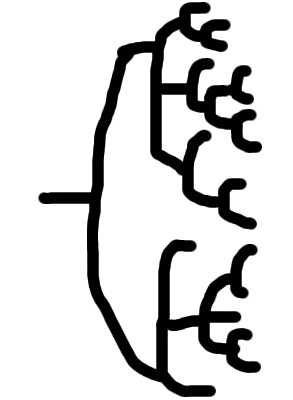
\includegraphics[scale=0.5]{img/diversidad-ling.png} 
\end{center}

\end{frame}

\begin{frame}{Diversidad lingüística: aumento de población}
\begin{itemize}
	\item No es ningún mérito que ahora haya más lenguas en el mundo que en épocas anteriores: nunca ha habido tanta población. 
	\item Acabamos de rebasar la cifra de 7.000M de habitantes. No rebasamos los 1.000M hasta principios del s. XIX. A principios del S. XX la población total era de 1.800M. 
	\item En los albores de la humanidad es posible que fuésemos menos de 1M en todo el globo.
	\item Es evidente que el número de lenguas ha ido creciendo a lo largo de los siglos y los milenios.
	\item A pesar del crecimiento exponencial de la población, no ha habido crecimiento exponencial del número de lenguas.
	\item De hecho, lo que ha ocurrido es que en un cortísimo espacio de tiempo:
	\begin{enumerate}
		\item han desaparecido centenares de lenguas: especialmente en América, Australia y Oceanía.
		\item algunas lenguas han aumentado mucho su número de hablantes.
	\end{enumerate} 
\end{itemize}
\end{frame}

\begin{frame}{Las familias lingüísticas}
\begin{itemize}
	\item Si las lenguas de hoy en día son divisiones de lenguas anteriores (y éstas, a su vez, divisiones de lenguas previas\ldots), ¿podemos llegar a la lengua de Adán y Eva?
	\item ¿Existió alguna vez una lengua única de la que se fueron separando todas las demás?
	\item Es una pregunta muy debatida y resulta imposible dar una respuesta definitiva, pero vale la pena echar un vistazo a cómo se agrupan las 5.000 ó 7.000 lenguas del mundo.
	\item Un primera aproximación para comparar lenguas es prestando atención a las semejanzas, justificadas por su parentesco. Es lo que se conoce con el nombre de \textcolor{blue}{clasificación genética}.
	\item Una \textcolor{blue}{familia lingüística} es un conjunto de lenguas genéticamente emparentadas que proceden de un ancestro común.
\end{itemize}

\end{frame}

\begin{frame}{El reparto de lenguas por el mundo}
\begin{itemize}
	\item Ya hemos visto que el reparto de lenguas por el mundo es desigual.
	\item La mayor diversidad lingüística se encuentra en África y en el Pacífico.
	\item A principios del s. XX, el ligüístia norteamericano Edward Sapir propuso la siguiente hipótesis:
	\begin{itemize}
		\item es de esperar que encontremos mayor diversidad lingüística en los emplazamientos más antiguos porque, lógicamente, ha habido más tiempo para la diversificación. 
	\end{itemize}
	\item Esta hipótesis coincide la Genética: la diversidad genética es tanto mayor cuanto más antigua sea la población.
	\begin{enumerate} 
		\item Hay más diversidad lingüística en Inglaterra que en EEUU, en España que en Latinoamérica.
		\item En el norte de África, hay más diversidad lingüística entre los pueblos bereberes (más antiguos) que entre la población de origen árabe (que es posterior).
	\end{enumerate} 
\end{itemize}
\end{frame}

\begin{frame}{Origen africano}
\begin{itemize}
	\item Si es cierta la correlación entre antigüedad y diversidad, África (el continente con mayor diversidad lingüística del mundo), tendrá también las lenguas más antiguas.
	\item Y si nos fijamos, dentro de África, en la zona geográfica con mayor concentración de lenguas distintas (actuales Camerún y Nigeria) haremos bien en poner el foco para tratar de buscar las lenguas más antiguas.
	\item Tradicionalmente, se suelen distinguir tres grandes familias lingüísticas africanas:
	\begin{itemize}
		\item khoisan: lenguas del sur y suroeste (actuales Angola, Namibia, Sudáfrica, etc.).
		\item afro-asiática: egipcio antiguo, árabe, hebreo, arameo, amhárico, etc.
		\item níger-kordofán: lenguas bantúes y sub-saharianas que no pertenecen a las dos lenguas anteriores.
	\end{itemize}
	\item Dentro de cualquiera de estas familias, la diversidad es aterradora. Algunas parecen diverger tanto como el chino y el español.
\end{itemize}
\end{frame}

\begin{frame}{Familias lingüísticas de África}

\begin{center} 
  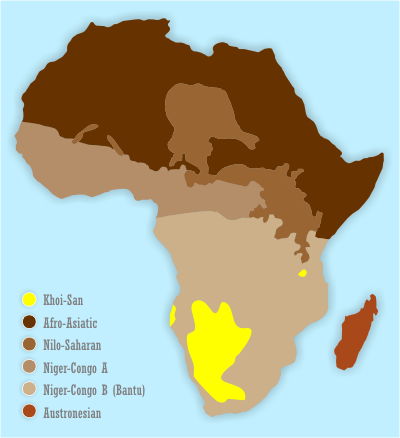
\includegraphics[scale=0.5]{img/lenguas-africa.png} 
\end{center}
\end{frame}


\begin{frame}{Familias lingüísticas de África}

\begin{center}
\begin{tabular}{ l l l l l l l }
   & \textbf{!kung} & \textbf{nama} & \textbf{hausa} & \textbf{maasai} & \textbf{zulú} & \textbf{swahili} \\
\hline
yo & mi & ti & ni & nanu & ami & mimi \\
tú & i & tsa & kai & inyi & akhu & ako \\
hablar & okx'ui & kx'ui & fada & iro & amb & amb \\
beber & k''a & kx'a & \ipa{\textesh\=a} & mat & phuza & nyw \\
ojo & \ipa{\textpipe ga} & mus & id\ipa{\=o} & \ipa{ongu} & so & cho \\
sol & \ipa{\textpipe am} & \ipa{\textpipe am} & rana & \ipa{olong} & \ipa{langa} & jua \\
\end{tabular}
\end{center}

\end{frame}


\begin{frame}{Las lenguas khoisan: hotentotes y bosquimanos}
\begin{itemize}
	\item Las lenguas de la familia khoisan son las lenguas de los pueblos tradicionalmente conocidos como hotentotes y bosquimanos.
	\item Geográficamente se extienden por las actuales Angola, Namibia, centro de Sudáfrica, Botswana y Zimbabwe, y un pequeño reducto en la actual Tanzania.
	\item Todas tienen una peculiaridad prácticamente exclusiva: los clicks o chasquidos, unas consonantes muy particulares.
	\begin{itemize}
		\item \href{http://www.youtube.com/watch?v=pGUzL2DVblc&feature=related\#}{Trabalenguas en xhosa}.
		\item \href{http://www.youtube.com/watch?v=gytCi5a7AJg}{Cliks en xhosa}
	\end{itemize}
	\pause
	\item Estos clicks, por muy extraños que parezcan, los usamos nosotros continuamente.
	\begin{itemize}
		\item [\ipa{\!o}] $\rightarrow$ click labial: es el sonido de un beso fuerte.
		\item [\ipa{//}] $\rightarrow$ click lateral: es el sonido para arrear a un caballo.
		\item [\ipa{!}] $\rightarrow$ click alveolar: es el sonido de descorchar una botella.
		\item [\ipa{|}] $\rightarrow$ click dental: es el sonido de un chasquido de disgusto.
	\end{itemize}
\end{itemize}
\end{frame}

\begin{frame}{Los clicks de las lenguas khoisan}
\begin{itemize}
	\item Más allá de la coincidencia superficial de los clicks, hay tanta diversidad entre las lenguas khoisan que sus hablantes no se entienden entre sí.
	\item Son lenguas habladas por pequeños grupos que han residido durante milenios en zonas colindantes.
	\item Es una familia lingüística bien reconocida que ha ocupado desde siempre el sur de África.
	\item Sus únicos familiares son otro par de lenguas de Tanzania, que también tiene clicks. 
	\item No sería extraño que la patria originaria estuviera precisamente en esa zona: los movimientos migratorios de los khoisan y los restos originarios del hombre moderno concuerdan con esta hipótesis.
	\item Los estudios genéticos y lingüísticos apuntan a la idea de que estos pueblos (y estas lenguas) están entre los descendients directos de los humanos modernos más antiguos.
\end{itemize}
\end{frame}

\begin{frame}{Tabla comparativa de distintas lenguas khoisan}

\begin{center}
\begin{tabular}{ l l l l l }
   & \textbf{\ipa{!kung}} & \textbf{\ipa{!xó\~o}} & \textbf{naron} & \textbf{nama} \\
\hline
yo & \ipa{mi} & \ipa{\textltailn'\textltailn} & \ipa{ti} & \ipa{ti} \\
tú & \ipa{i} & \ipa{\=ah} & \ipa{satSa} & \ipa{tsa} \\
hablar & \ipa{okx'ui} & \ipa{tana} & \ipa{!gava} & \ipa{kx'ui} \\
beber & \ipa{k''a} & \ipa{kx'\=ah\~a} & \ipa{k''a} & \ipa{kx'a} \\
ojo & \ipa{\textpipe ga} & \ipa{\textpipe 'u\~i} & \ipa{mùs} & \ipa{m\~us} \\
sol & \ipa{\textpipe am} & \ipa{\textpipe \textpipe 'an} & \ipa{\textpipe amSa} & \ipa{\textpipe am} \\
\end{tabular}
\end{center}

\end{frame}


\begin{frame}{Diversidad lingüísitca en otras zonas del mundo}
\begin{itemize}
	\item Recapitulando, podemos demostrar desde un punto de vista genético y arqueológico que el lugar con la población más antigua es África.
	\item El lugar con mayor diversidad lingüística es África.
	\item Las lenguas de la familia khoisan están entre las más antiguas de África.
	\item Hasta ahora diversidad $\approx$ antigüedad. ¿Sirve esa ecucación para explicar la diversidad lingüística de otras zonas del mundo?
	\item Tras África, los asentamientos más antiguos del hombre modernos (hacia el 60.000 aC) son el sureste asiático y Papúa Nueva Guinea.
	\item La ocupación de Asia, Europa y América sería más reciente, y eso se refleja en la menor diversidad lingüística.  
\end{itemize}
\end{frame}


\begin{frame}{Migraciones humanas}
\begin{center} 
  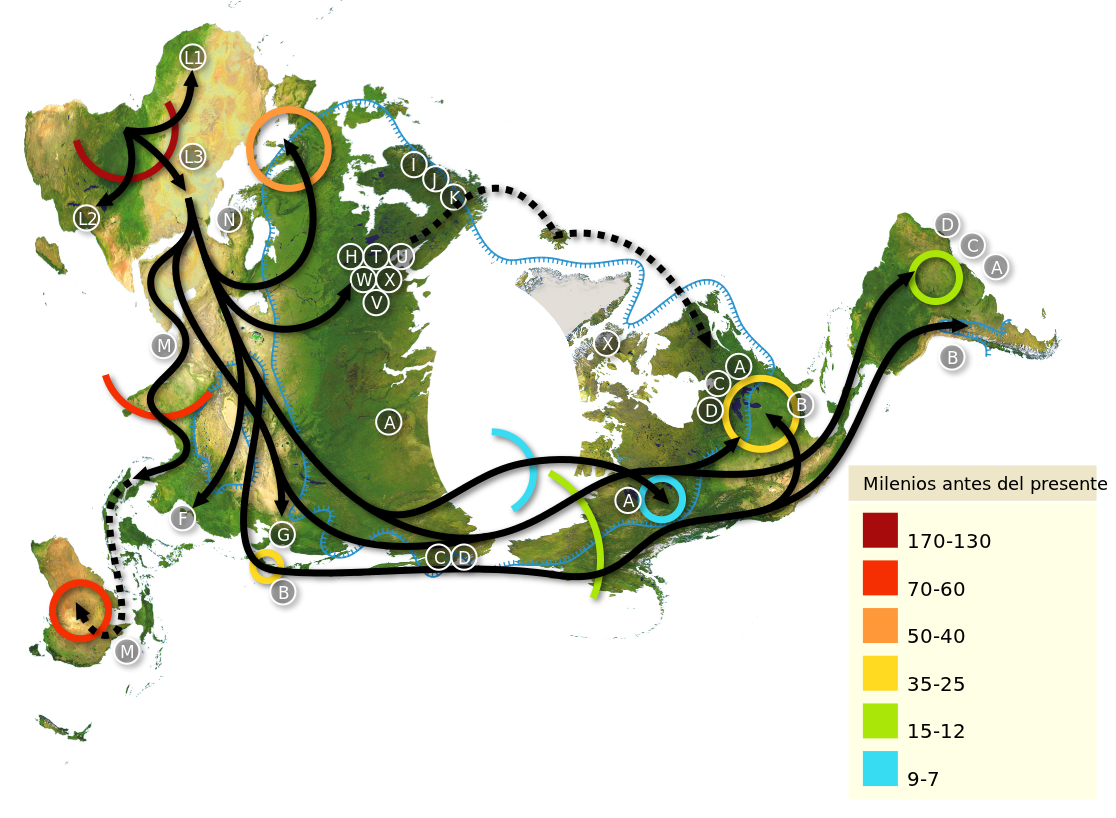
\includegraphics[scale=0.35]{img/Migraciones_humanas.png} 
\end{center}\end{frame}


\begin{frame}{Lenguas de América}
\begin{itemize}
	\item La ocupación de América es posterior al de otras zonas del mundo, sin embargo, la diversidad lingüística parece indicar que se ocupó en diversas oleadas.
	\item Si comenzamos por el final, los inuit (esquimales) fueron la última migración hace unos pocos milenios. Se encontraron todo el continene ocupado y, en consecuencia, decidieron quedarse en el extremo norte, desde Alaska hasta Groenlandia (familia esquimo-aleutiana).
	\item Un tiempo antes, hace 5.000 - 10.000 años, habían llegado por el mismo camino otros pueblos. Se encontraron las tierras del sur ocupadas, así que se extendieron por la franja noroccidental de los actuales EEUU y Canadá y en el centro-sur de EEUU (familia na-dene).
	\item Antes que ellos, otros pueblos fueron llegando a América y se encontraron un continente prácticamente vacío. Pudieron extenderse desde norteamérica hasta Tierra del Fuego con bastante rapidez (familia amerindia).
	
\end{itemize}
\end{frame}


\begin{frame}{Lenguas indoeuropeas}
\begin{itemize}
	\item Dejando aparte la reciente expansión del francés, inglés, portugués, neerlandés u español existe un grupo de lenguas que ha ocupado un extenso territorio desde hace mucho tiempo: las \textcolor{blue}{lenguas indoeuropeas}.
	\item El parentesco de estas lenguas se estableció desde finales del s. XVIII. Véase el \href{http://upload.wikimedia.org/wikipedia/commons/4/4f/IndoEuropeanTree.svg}{árbol genealógico}.
	\item Al principio, se consideraban integrantes de esta familia las lenguas románicas («hijas del latín») el griego, las germánicas, las eslavas, las bálticas (lituano y letón), célticas, iranias e indias (como el sánscrito).
	\item Posteriormente, se han ido uniendo otras lenguas cuyo parentesco no resultaba tan evidente: albanés, armenio, lenguas desaparecidas de la península itálica (osco-umbro, etrusco) y los Balcanes (tracio, ilirio), lenguas de China (tocario) y de Anatolia (hitita). 
\end{itemize}
\end{frame}


\begin{frame}{Tabla comparativa de diversas lenguas indoeuropeas}
\begin{center}
\begin{footnotesize}
\begin{tabular}{ l l l l l l l l }
 & \textbf{yo} & \textbf{tú} & \textbf{¿quién?} & \textbf{agua} & \textbf{nombre} & \textbf{muerte} & \textbf{dos} \\
\hline
latín & ego & tu & quis & - & nomen & mortuus & duo \\
griego & ego & su & tis & hudor & onoma & ambrotos & duo \\
gótico & ik & \ipa{\th u} & hwas & wato & namo & \ipa{mor\th r} & twe \\
lituano & \ipa{aS} & tu & kas & vanduo & emmens & mirti & du \\
eslavo & azu & ty & kuto & voda & ime & mrto & duo \\
sánscrito & ahám & tuvám & kas & udakám & naman & mrtá & duv \\
tocario & - & twe & kuse & war & \ipa{\textltailn em} & - & wi \\
hitita & uk & - & kuis & watar & laman & merta & twi \\
\end{tabular}
\end{footnotesize}
\end{center}
\end{frame}


\begin{frame}{Los pueblos indoeuropeos}
\begin{itemize}
	\item ¿De dónde y cuándo salió esta familia? Existen varias teorías.
	\item Lo que se conoce como la hipótesis estándar defiende que los indoeuropeos serían un pueblo de la edad de cobre dedicado al pastoreo que había domesticado el caballo.
	\item Habitaron las estepas del Cáucaso, el sur de Rusia y Ucrania entorno al año 3.000 aC. Desde ahí se fueron extendiendo:
	\begin{itemize}
		\item Primero se separaron los anatolios. 
		\item Después, hacia el suroeste, los griegos, tracios, ilirios, itálicos.
		\item Hacia el oeste, los celtas, con los germanos, bálticos y eslavos, que se dirigieron hacia el noroeste.
		\item Hacie el sureste, se fueron los indo-iranios y un poco hacia el noreste, los tocarios. 
	\end{itemize}
	\item Así fueron extendiéndose y, tras mezclarse con pueblos aborígenes de los nuevos asentamientos, dieron lugar a las lenguas actuales.
\end{itemize}
\end{frame}


\begin{frame}{Agrupación de lenguas en el mundo}

A continuación se detalla una hipótesis atrevida sobre la agrupación de las lenguas del mundo, con «solo» 12 grandes familias.

\begin{itemize}
	\item \textcolor{blue}{khoisán}: África meridional.
	\item \textcolor{blue}{níger-cordofán}: centro de África, de costa a costa. 
	\item \textcolor{blue}{nilo-sahariana}: sur de Sudán y centro-este de África.
	\item \textcolor{blue}{afro-asiática}: norte de África, Etiopía, península arábiga.
	\item \textcolor{blue}{euro-asiática}: casi toda Europa (excepto euskera y lenguas caucásicas), buena parte de Asia, Alaska y Groenlandia.
	\item \textcolor{blue}{kartvelia}: georgiano y lenguas del Cáucaso.
\end{itemize}
\end{frame}

\begin{frame}{Agrupación de lenguas en el mundo: hipótesis atrevida}
\begin{itemize}
	\item \textcolor{blue}{áustrica}: lenguas de Indochina, Taiwán, Madagascar, Filipinas, Indonesia y Polinesia.
	\item \textcolor{blue}{dravídica}: mitad sur de India, norte de Sri Lanka y zona oeste de Pakistán.
	\item \textcolor{blue}{indo-pacífico}: Papúa Nueva Guinea y las lenguas extintas .
	\item \textcolor{blue}{australiana}: lenguas aborígenes de Australia.
	\item \textcolor{blue}{amerindia}: casi toda América, de norte a sur.
	\item \textcolor{blue}{dene-caucásica}: lenguas sino-tibetanas (variantes del Chino), lenguas del Caúcaso, lenguas na-dene de Norteamérica, lenguas del Yenisei\ldots y el euskera.
\end{itemize}
\end{frame}

\begin{frame}{Familias lingüísticas del mundo}
\begin{center} 
  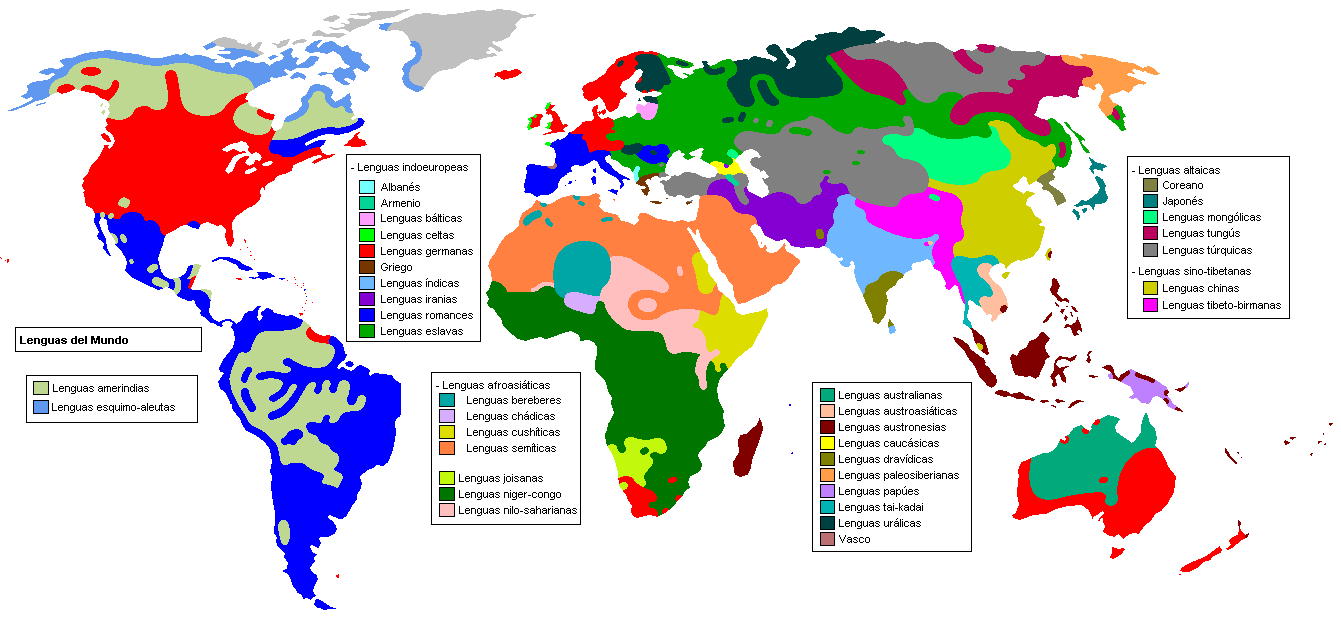
\includegraphics[scale=0.25]{img/lenguas-mundo.png} 
\end{center}

\end{frame}

\begin{frame}{Tres escenarios para una primera lengua}

\begin{itemize}
	\item Es imposible saber si alguna vez existió una única lengua. Pero podemos presentar tres escenarios distintos.

\begin{enumerate}
	\item El lenguaje surge cuando toda la humanidad moderna vive en África. Con el paso del tiempo, las poblaciones se mueven y se separan, y con ellas sus lenguas.
	\item Igual que el segundo escenario, pero con muchos contactos posteriores entre grupos, de manera que poblaciones que emigran vuelven al punto de origen y se mezclan con los «sus primos».
	\item El lengua va surgiendo como consecuencia de las necesidades de la población en movimiento y en constante adaptación. Las lenguas surgen sin relación unas con otras.
\end{enumerate}
	\item Los tres escenarios permitirían el mismo resultado final: la actual diversificación de lenguas.
\end{itemize}

\end{frame}


\begin{frame}{En busca de la «lengua madre»}
\begin{itemize}
	\item Ha habido diferentes intentos de encontrar la lengua madre o el ancestro común mas antiguo.
	\item Las lenguas que conocemos actualmente no son demasiado antiguas: el chino, el sumerio, el hitita, no tienen más de 5.000 años.
	\item No tenemos registro de lenguas antiguas, Necesitamos recurrir a un método que nos permita reconstruir los restos de esas proto-lenguas.
	\item A partir de estudios comparativos y teniendo en cuenta la evolución y el cambio lingüístico reciente podemos reconstruir la base lingüística (no tanto palabras reales) de la que surgen las palabras de las lenguas actuales.
	\item Illich-Svitych trató de de encontrar los rastros de una antiquísima «lengua tatarabuela» a la que llamó nostrático.
	\item Greenberg a través de un método comparativo, multilateral ha propuesta una proto-lengua llamada euroasiático.
\end{itemize}
\end{frame}

\begin{frame}{}
\begin{center}
\LARGE Clasificación tipológica de las lenguas 
\end{center}
\end{frame}

\begin{frame}{Clasificación tipológica de las lenguas}
\begin{itemize}
	\item La clasificación genética no es la única forma de comparar y relacionar las lenguas del mundo.
	\item Existe la posibilidad de agrupar las lenguas en base a determinadas características estructurales y sin antender a su parentesco. 
	\item Es lo que se conoce con el nombre de \textcolor{blue}{clasificación tipológica} y analiza las siguientes características estructurales de las lenguas:
	\begin{itemize}
		\item estructura verbal.
		\item sistema fonológico (sonidos vocálicos y consonánticos).
		\item estructura de la palabra.
		\item orden habitual de los elemenos de la oración.
	\end{itemize}
\end{itemize}
\end{frame}

\begin{frame}{Estructura de la palabra: lenguas sintéticas vs. lenguas analíticas}

Atendiendo a la estructura habitual de las palabras, la clasificación tipológica suele dividir las lenguas del mundo bajo dos categorías distintas: 

\begin{itemize}
	\item las \textcolor{blue}{lenguas sintéticas} se caracterizan porque sus palabras están constituidas por varios morfemas distintos. En estas lenguas existen mecanismos para crear significados complejos por medio de flexión y derivación.
	
	Son típicas lenguas sintéticas las indoeuropeas (latín, griego, romances, sánscrito, ruso, alemán), las lenguas dravídicas y algunas americanas (quechua, navajo, náhuatl).
	
	\item las \textcolor{blue}{lenguas analíticas} se caracterizan porque sus palabras son monomorfemáticas. Es decir, no tienen mecanismos de flexión ni derivación y las palabras complejas son resultado de procesos de composición. 
	
	Típicas lenguas analíticas son el chino y las lenguas aústricas.   
	
\end{itemize}
\end{frame}

\begin{frame}{Tipos de lenguas sintéticas}

Las lenguas sintéticas, a su vez, suelen dividirse en dos grandes grupos, dependiendo del mecanismo de creación de palabras más frecuente.

\begin{itemize}
	\item las \textcolor{blue}{lenguas flexivas} son aquellas cuyas palabras suelen estar formadas por más de un morfema que, a su vez, es capaz de sintetizar información de distintas categorías. 
	
	Ejemplos típicos de lenguas flexivas son el latín, griego, ruso y todas las lenguas romances.
	
	\item las \textcolor{blue}{lenguas aglutinantes} son aquellas cuyas palabras suelen estar formadas por más de un morfema, cada uno de ellos aporta un tipo de significado diferente (léxivo, derivatibavo, gramatical). 

	Ejemplos típicos de lenguas aglutinantes son el turco, el finés y el euskera.

\end{itemize}
\end{frame}

\begin{frame}{Estructura de palabras en español}

Anque el español es mayoritariamente una lengua sintética de tipo flexivo, podemos encontrar ejemplos de palabras típicos de otros tipos de lenguas.

\begin{itemize}
	\item \textit{cant-o} tiene dos constituyentes. El morfema \textit{cant-} aporta el significado léxico y el morfema \textit{-o} sintetiza información de distintas categorías: modo indicativo, tiempo presente, primera persona, número singular. Es un ejemplo típico de las \textcolor{blue}{lenguas flexivas}.

	\item \textit{granj-er-a-$\varnothing$} tiene cuatro constituyentes. El el morfema \textit{granj-} aporta el significado léxico («casa de labranza»), \textit{-er-} aporta el significado derivativo («persona o cosa relacionada con el lugar anterior»), \textit{-a-} aporta el significado gramatical relativo a género femenino y el morfema $\varnothing$ indica el número. Es un ejemplo típico de las \textcolor{blue}{lenguas aglutinantes}.

\end{itemize}
\end{frame}

\begin{frame}{Estructura de palabras en español}

\begin{itemize}
	\item \textit{rompe-cabezas} tiene dos constituyentes. Dos elementos independientes se han unido para formar una palabra compuesta. Es un ejemplo típico de las \textcolor{blue}{lenguas analíticas}.

\end{itemize}
\end{frame}

\begin{frame}{Orden oracional}

\begin{itemize}
	\item La clasificación tipológica también se aplica a la investigación del orden canónico de los elementos oracionales en las distintas lenguas.
	\item En muchas lenguas el orden de los elementos oracionales no es fijo, aunque siempre hay un orden no marcado.
	\item Podemos establecer los siguientes tipos de lenguas atendiendo al orden de aparición del sujeto (S), el verbo (V) y el objeto (O):
	\begin{itemize}
		\item  lenguas SOV: euskera, latín y griego clásico, árabe, japonés, hindi, sánscrito, turco, alemán (con verbos compuestos), nóstrático
		\item lenguas SVO: castellano, inglés, francés, italiano, chino mandarín, griego moderno, swahili
		\item lenguas VSO: galés, tagalo 
		\item También hay lenguas con orden VOS (malgache, javnés, fiyiano) y OVS (interlingua, klingon).
	\end{itemize}
\end{itemize}
\end{frame}

\begin{frame}{Orden oracional}
\begin{itemize}
	\item Las lenguas SOV y SVO representan alrededor del 75\% de las lenguas del mundo. 
	\item Las lenguas SOV comparten las siguientes características:
	\begin{itemize}
		\item Tendencia a las postposiciones frente a las preposiciones.
		\item Las oraciones de relativo y los adjetivos suelen preceder al nombre que modifican. 
		\item En general, el orden habitual del elementos en el sintagma es modificador + núcleo.
	\end{itemize}
	\item Por su parte, las lenguas SVO presentan las siguientes características:
	\begin{itemize}
		\item Tendencia a las preposiciones frente a las postposiciones.
		\item Las oraciones de relativo y los adjetivos se situán detrás del nombre al que modifican (antecedente).
		\item En general, el orden habitual del elementos en el sintagma es núcleo + modificador.
	\end{itemize}\end{itemize}

\end{frame}
	


\begin{frame}{}
\begin{center}
\LARGE El paso del tiempo y el cambio lingüístico 
\end{center}
\end{frame}

\begin{frame}{Desaparición de una lengua}
\begin{itemize}
	\item Las lenguas pueden desaparecer. No tiene que pasar necesariamente, hay lenguas que existen (con muchos cambios, eso sí) dede hace miles de años.
	\begin{itemize}
		\item El chino es chino desde hace más de 4.000 años.
		\item El hindi actual es la continuación de antiguas lenguas indias.
		\item Castellano, gallego y catalán son continuación del latín, que a su vez es continuación del indoeuropeo, que es continuación de\ldots.
	\end{itemize}
	\item Podemos entender «desaparición» de dos formas distintas:
	\begin{enumerate}
		\item la desaparición completa de una lengua: antes existía y ahora no.
		\item la desaparición aparente de una lengua, debido al paso del tiempo y al cambio lingüístico.
	\end{enumerate}
\end{itemize}
\end{frame}

\begin{frame}{Desaparición de una lengua}

\begin{itemize}
	\item Existe constancia de la desaparición de lenguas en muchos países y en todas las épocas: 
	\begin{itemize}
		\item En la Isla de Man, en Reino Unido, hace menos de 100 años se hablaba el manx. Ya no quedan hablantes nativos. En 1777 murió el último hablante de cornuallés.
		\item En España desaparecieron el ibérico y todas las lenguas célticas que se hablaban antes de la llegada de los romanos.
		\item En Italia desaparecieron el osco, el etrusco y el venético.
		\item En Oriente medio se hablaron lenguas como el hitita y el sumerio. No se hablan desde hace miles de años, solo nos quedan textos escritos en tabillas de barro.
		\item En América y Australia la desaparición de lenguas fue de la mano de la desaparición de los pueblos indígenas que las hablaban.
		\item En otras ocasiones, por fortuna, las lenguas mueren simplemente porque sus hablantes deciden dejar de utilizarlas. 
	\end{itemize}
\end{itemize}
\end{frame}

\begin{frame}{La muerte de lenguas en EEUU}
\begin{itemize}
	\item Conocemos bastante bien la reciente y continuada desaparición de lengua indias en EEUU.
	\item Las poblaciones indias fueron reducidas en número, desplazadas de su lugar de origen y relegadas en reservas.
	\item Desde finales del x. XIX la política gubernamental intento la asimilación: los niños eran educados en internados, en inglés
	\item Se calcula que el 80\% de las lenguas de EEUU y Canadá desaparecerán en breve plazo.
\end{itemize}

\begin{center}
\begin{footnotesize}
\begin{tabular}{ l r r }
\textbf{lengua} & \textbf{hablantes} & \textbf{población} \\
\hline
powahatan & 0 & 3.500 \\
comanche & 854 & 6.000 \\
cheyenne & 1.721 & 5.000 \\
hopi & 5.265 & 6.500\\
apache & 15.333 & 20.000\\
sioux dakota & 16.000 & 100.000\\
cherokee & 23.000 & 300.000 \\
navajo & 150.000 & 220.000 \\
\end{tabular}
\end{footnotesize}
\end{center}

\end{frame}

\begin{frame}{La muerte de lenguas en EEUU}
\begin{itemize}
	\item De las 159 lenguas indias de EEUU, solo 36 tienen más de 1.000 hablantes nativos.
	\item La inmensa mayoría de estas lenguas no se ha usado nunca en la escritura, o solo desde hace poco tiempo.
	\item Cuando hay suficiente número de hablantes, es posible tomar la decisión de utilizar la lengua de manera que pueda aprenderla la nueva generación: hablándola en casa, en la vida cotidiana y en la escuela.
	\item En EEUU hay otras lenguas minoritarias no indias que no corren ningún peligro: el \it{canjun french} de Luisiana o el \it{pennsylvania dutch} de los amish $\rightarrow$ dos poblaciones con una clara identidad étnico-cultural o religiosa.
	\item El desarraigo de los indios les ha hecho perder gran parte de su cultura tradicional.
	\item A pesar del actual proceso de revitalización de las culturas indias, la desventaja de la que parten las lenguas es evidente y su recuperación compleja.
\end{itemize}
\end{frame} 

\begin{frame}{En todas partes mueren lenguas}

\begin{itemize}
	\item No solo en los países de habla inglesa desaparecen lenguas.
	\item El 25\% de las lenguas indias de Latinoamérica están en peligro de extinción inmediata.
	\item Aunque la mayoría de estas lenguas no corre peligro desde el pdv demográfico, sí lo corre por motivos de prestigio social. 
	\item Con expeción del guaraní (lengua co-oficial en Paraguay), el resto de lenguas suelen ser despreciadas por ser «cosa de indios».
\end{itemize}
\begin{center}
\begin{footnotesize}
\begin{tabular}{ l r l }
\textbf{lengua} & \textbf{hablantes} & \textbf{país} \\
\hline
cayapa & 5.000 & Ecuador\\
yanomami & 15.000 & Venezuela, Brasil \\
mapuche & 400.000 & Chile\\
náhuatl & 1.380.000 & México \\
aymara & 2.200.000 & Bolivia, Perú, Chile\\
lenguas mayas & 3.000.000 & Guatemala, México, Belize \\
guaraní & 4.650.000 & Paraguay \\
quechua & 8.000.000 & Bolivia, Perú, Ecuador, Colombia\ldots \\
\end{tabular}
\end{footnotesize}
\end{center}

\end{frame}

\begin{frame}{Lenguas que resucitan}
\begin{itemize}
	\item Pero las lenguas pueden resucitar.
	\item El hebreo dejó de ser una lengua hablada y quedó limitada a su uso en ritos religioso durante siglos. 
	\item Durante el s. XX, con la creación del estado de Israel, su uso se revitalizó y goza de muy buena salud.
	\item En España, el euskera nunca no dejó de tener hablantes aunque su uso quedó muy limitado a áreas rurales. 
	\item Como hemos visto anteriormente, los mecanismos de normativización y normalización lingüística suelen venir acompañados de la introdución de la lengua minoritaria en la escuela a todos los niveles.
	\item Para reforzar, impulsar, revitalizar o resucitar cualquier lengua hay que establecer incentivos para que la gente la use en todas las situaciones posibles.
\end{itemize}
\end{frame}


\begin{frame}{}
\begin{center}
\LARGE ¿Hay lenguas mejores y peores? ¿Más o menos primitivas? 
\end{center}
\end{frame}

\begin{frame}{}
\begin{itemize}
	\item Los no lingüistas (y a veces, algunos lingüista también) hablan a menudo de «lenguas primitivas» y las clasifican en mejores y peores $\rightarrow$ volvemos a la distinción entre lengua y dialecto.
	\item Se suele hablar de «lenguas con gramática» y «lenguas sin gramática». Esto es un sinsentido, la gramática es un componente esencial del lenguaje humano.
	\item Este tipo de afirmaciones puede venir de la creencia falsa de que «tener gramática» consiste en «tener una variante estándar» o tener tradición literaria escrita.
	\item El origen de todas estas ideas está en la época colonial, cuando interesaba dejar bien clara la diferencia entre los pueblos civilizados europeos y los pobres e ignorantes salvajes.
	\item Todas las lenguas que existen, han existido o puedan existir en el futuro tienen gramática.
	\item No se conoce ningún pueblo que haya carecido de algo semejante a nuestra literatura, aunque no esté escrita. 
\end{itemize}
\end{frame}


\begin{frame}{Breve inmersión en las lenguas khoisan}
\begin{itemize}
	\item Ya hemos visto que las lenguas khoisan están probablemente entre las lenguas más antiguas del mundo. 
	\item ¿Son lenguas primitivas o inferiores? ¿Comparadas con qué? Echemos un vistazo al vocabulario para ver qué significados son capaces de trasmitir.
	\begin{itemize}
		\item \ipa{[g\!ohx'ó\~o]}: mosca
		\item \ipa{[dts'kx'\=ala]}: olor a pradera quemada
	\end{itemize}
	\item La característica principal de esta familia de lenguas es el uso de los sonidos clicks que aparecen en el 60\% de sus palabras.
	\item Estos clicks tienen en cierta medida semántica: hay cierta relación entre el sonido y ciertas ideas generales:  
	\begin{itemize}
		\item click alveolar lleva asociado significado de `algo abombado'.
		\item click lateral parece corresponder con la idea de `algo alargado y grueso'
		\item click dental es predominante la idea de algo `largo y flexible'.
		\item click palatal lleva asociado la idea de `algo espeso y denso'.
		\item click labial indica `conjunto de cosas individuales y juntas'.
	\end{itemize}
\end{itemize}
\end{frame}


\begin{frame}{Breve inmersión en las lenguas khoisan}
\begin{itemize}
	\item Los san tienen muchas palabras distintas para indicar cosas que nosotros entendemos como unitarias.
	\begin{itemize}
		\item llevar: llevar a un niño en la cadera \ipa{[|gâm]}; llevar apretado contra el pecho \ipa{[gàh'o]}; llevar colgado de un palo al hombro \ipa{[||gàlo]}; llevar apoyado contra el hombro \ipa{[!án]}; llevar sobre la cabeza \ipa{[!ú\~u //àm]}; llevar un contenedor de líquido \ipa{[//nùh\~a]}.
		\item beber: beber un líquido caliente \ipa{[sàm]}; beber un líquido frío \ipa{[qôm]}; arrodillarse para coger el agua \ipa{[//qàm]}; beber sorbiendo de un huevo de avestruz \ipa{[\!ogùmi]}; beber hasta quedar satisfecho \ipa{[d\=oh'o]}
		\item estar tumbado: horizontal; al acecho; sobre una esterilla; sobre la espalda; boca abajo; de costado para resistir mejor el hambre.
		\item caminar: de aquí para allá; como un enfermo; sobre las huellas de otra persona; sobre algo húmedo; sobre las puntas de los pies; en fila india; haciendo crugir las rodillas.
	\end{itemize}
	\item Estos matices son un claro reflejo de sus necesidades de comunicación: son un pueblo cazador-recolector. 
\end{itemize}

\end{frame}

\begin{frame}{Breve inmersión en las lenguas khoisan}
\begin{itemize}
	\item Los san que viven aún a la manera tradicional tienen pocos temas de conversación comparados con los nuestros, pero cuando les conviene son muy precisos.
	\item Primitivismo no, especialización sí, aunque sus campos de especialización nos parezcan poco tecnológicos.
	\item Si nos fijamos en la gramática, vemos que las lenguas khoisan tienen subordinación y voz pasiva.
	\item También distinguen singular y plural, no solo en los sustantivos sino también en los verbos.
	\item En castellano hay dos géneros (masculino y femenino) y dos números (singular y plural). Las lenguas san tienen cinco clases de sustantivos que pueden ser singulares o plurales. Todas estas formas tienen concordancia.
	\item No hay nada realmente primitivo, ni supuestamente inferior o menos complejo en las lenguas khoisan que en otras.
\end{itemize}

\end{frame}

\begin{frame}{El progreso lingüístico}
\begin{itemize}
	\item Durante parte del s. XIX se creía en un proceso que conducía de lo simple a lo complejo.
	\item Se tomaba como lenguas cercanas a la perfección el latín, el griego y el sánscrito porque tenían casos, numerosísimas formas verbales.
	\item A más complicación, más perfección.
	\item Está claro que las culturas han ido evolucionando haciéndose cada vez más complejas. La cultura occidental es más compleja que la bosquimana. Pero eso no tiene nada que ver con las lenguas.
	\item Por mucho que busquemos, no encontraremos ninguna lengua (viva, muerta o moribunda, moderna o antigua) que no tengan cosas que no existen en otras lenguas.
	\item Todas las lenguas iguales a sus capacidades de uso.
\end{itemize}

\end{frame}

\begin{frame}{La complejidad estructural de las lenguas}

\begin{itemize}
	\item La única forma de medir la complejidad estructural de las lenguas es teniendo en cuenta el esfuerzo mental implicado en el procesamiento es esas estructuras.
	\item En quechua es más sencillo formar el plural que en latín.
	\begin{itemize}
		\item En quechua basta con añadir -kuna al final de cualquier sustantivo.
		\item En latín depende de la declinación. \it{dominus} tiene plural \it{domini}, \it{rosa} tiene plural en \it{rosae}, \it{templum} tiene plural \it{templa}. 
	\end{itemize}
	\item La construcción aglutinante (como el quechua) es cognitivamente menos costosa que la flexiva (como el latín).
	\item A menor morfología, menor complicación. Pero en las lenguas sin morfología, las complicaciones vienen del lado de la sintaxis.
	\item Una vez más, aunque seamos capaces de definir complejidad estructural, no tiene ningún significado en términos valorativos.
	\item Todas las lenguas tienen aspectos sencillos y aspectos complejos. 
\end{itemize}

\end{frame}


\begin{frame}{}
\begin{center}
\LARGE Lenguas pidgin y lenguas criollas 
\end{center}
\end{frame}


\begin{frame}{Contexto histórico}
\begin{itemize}
	\item Durante la epoca colonial, comerciantes de esclavos europeos se reúnen en la costa de África occidental.
	\item Los esclavos proceden de distintas zonas y hablan lenguas distintas. No se pueden comunicar en sus lenguas nativas.
	\item Los esclavistas hablan distintas lenguas también. Utilizan como lengua de intercambio el inglés o el portugués. La mayoría como lengua aprendida, así que la conocen mínimamente. Los hablantes nativos son gente de escasa educación. 
	\item Los esclavos son «almacenados» todos juntos. Para evitar motines, se procura separar a los proceden de la misma tribu.
	\item No hay lengua común, pero el ser humano es incapaz de vivir sin comunicarse, aunque sea de forma elemental.
		\begin{itemize}
			\item Los negreros necesitan dar órdenes, discutir de negocios.
			\item Los esclavos necesitan comunicarse entre ellos y entender a los negreros.
		\end{itemize}
\end{itemize}

\end{frame}

\begin{frame}{Los pidgin}
\begin{itemize}
	\item En una situación como la descrita, basta con tener un «pedacito de lengua»: el vocabulario imprescindible para tratar los temas necesarios, una gramática mínima que sea fácil de aprender, una pronunciación simplificada.
	\item La palabra \it{pidgin} (hispanizada como piyin) proviene de la pronunciación china de \it{business}.  
	\item Los pidgin son «medias lenguas» y no sirven para mucho, solo para «hablar de negocios».
	\item En situaciones en las que resulta imprescindible encontrar una lengua para negociar se suelen recurrir a estos esqueletos lingüístico de escaso vocabulario.
	\item No solo surgieron pidgin en el escenario de la trata de esclavos. Hubo pidgin en el Mediterráneo medieval (la lingua franca), en el Ártico (el russenorsk), en la frontera ruso-china, entre comerciantes ingleses y empleados cantoneses, en las islas del Pacífico, entre colonos y balleneros con los indios de Norteamérica.
\end{itemize}

\end{frame}

\begin{frame}{Los pidgin}
\begin{itemize}
	\item Se aprenden fácilmente y sirven para salir del paso y solucionar las necesidades de comunicación más cotidianas.
	\item ¿Cómo son estos pidgin? 
	\begin{itemize}
		\item No existe apenas morfología, las palabras van unas detrás de las otras sin marcar ningún tipo de concordancia.
		\item Tampoco hay muchas reglas sintácticas. La comprensión depende mucho del interés que pongan los interlocutores.
		\item Suelen constar de una mezcla de sintaxis simplificada y vocabulario de la lengua europea, con vocabularios de otras lenguas africanas.
	\end{itemize}
	\item Pasa el tiempo, comienza la travesía hacia América y el Caribe y, a bordo, solo existe el pidgin.
	\item Llegan a las plantaciones, se mezclan unos esclavos con otros y solo existe el pidgin.
	\item Con el paso del tiempo, este pidgin va enriqueciendo su vocabulario con palabras de las lenguas de los señores.
\end{itemize}

\end{frame}

\begin{frame}{Criollización de los pidgin}

\begin{itemize}
	\item Pasa el tiempo y nacen niños, inmersos en una comunidad sin lengua propia.
	\item Los niños se crían rodeados de lenguas africanas distintas. Escuchan el pidgin que se utiliza como lengua común y también la lengua europea de los señores.
	\item ¿Qué lengua podrían hablar estos niños?
	\begin{itemize}
		\item Están poco expuestos a las lenguas europeas como para convertirse en nativos de inglés, español o portugués.
		\item Las lenguas africanas se hablaban a escondidas, tampoco pueden llegar a aprenderlas adecuadamente.
		\item La única posibilidad es el pidgin pero, como hemos visto, este pidgin no soluciona todas las necesidades de comunicación.
	\end{itemize}
	\item Ese pidgin que escuchan a los adultos es bastante más rico que el que se originó en África. Los niños van añadiendo poco a poco nuevo vocabulario de aquí de allá y crean reglas sintácticas que se adaptan a sus necesidades.  
\end{itemize}
\end{frame}

\begin{frame}{Criollización de los pidgin}

\begin{itemize}
	\item En un plazo relativamente corto aquel pidgin se ha convertido en una lengua completa a todos los efectos: un criollo.
	\item Si hace falta una palabra nueva se toma prestada o se inventa (como hace cualquier lengua).
	\item Este proceso de criollización está bien estudiado. En cuestión de dos generaciones apareció la lengua criolla de la Guayana Holandesa (hoy Surinam). 
	\begin{itemize}
		\item Las plantaciones estaban en manos de los ingleses. 
		\item Los primeros esclavos crearon un pidgin básico. 
		\item Sus hijos, una generación después, crearon un criollo con base en inglés: el sranan tongo (\it{surinam tongue}).
	\end{itemize}
\end{itemize}
\end{frame}

\begin{frame}{Pidgin y criollos en el mundo}

\begin{itemize}
	\item No todos los pidgin ni todos los criollos tienen como base el inglés. 
	\item En la isla de Anobón, en Guinea Ecuatorial, se habla la fa d'Ambó: un criollo con base en portugués.
	\item El chabacano es un criollo de base española hablado todavía en el sur de Filipinas.
	\item En las Antillas Holandesas la lengua oficial es el papiamento: un criollo de base portuguesa relexificado a español.
	\item Esta relexificación es muy habitual, cuando las plantaciones cambiaban de manos.
	\begin{enumerate}
		\item De la frase originaria en español: \it{Quiero ir a comer, ¿vienes tú también?}
		\item Se genera un pidgin del estilo: \it{mi querer comer ¿tú venir también?}
		\item Y se relexifica al inglés: \it{me want go eat, you come too?}
		\item La pronunciación se simplifica: \it{mi wan go it, yu kam tu?}
	\end{enumerate}
\end{itemize}
\end{frame}

\begin{frame}{Características de los criollos}
\begin{itemize}
	\item El orden de los elementos oracionales tiende a fijarse. El oyente agradecerá no tener que preocuparse por el orden de palabras.
	\begin{itemize}
		\item El papiamento prefiere el orden SVO. Cuando hay que poner algo en relieve, el papiamento utiliza construcciones extrapuestas.
		\item \it{El castellano lo hablo bien} sería en papiamento \it{ta casteyano mi ta papia bene} «es castellano lo que hablo bien».
	\end{itemize}
	\item La persona no se expresa en el verbo, sino con un pronombre que aparece obligatoriamente.
	\begin{itemize}
		\item español: \it{vengo, vienes, viene, venimos, venís, vienen}
		\item papiamento: \it{mi ta beni, bo ta beni, e ta beni, nos ta beni, bos ta beni, nan ta beni}
		%\item inglés: \it{I come, you come, he comes, we come, you come, they comer}
		\item neerlandés: \it{ik koom, jij koomt, hij koomt, wij koomen, jullie koomt, zij komen}
		\item africaans: \it{ek koom, jy koom, hy koom, ons koom, jul koom, sy koom}
		\item chino: \it{wo lai, ni lai, ta lai, women lai, nimen lai, tamen lai}
	\end{itemize}
\end{itemize}
\end{frame}

\begin{frame}{Características de los criollos}
\begin{itemize}
	\item Los tiempos se limitan en número y, a veces, se transforman en aspectos (en lugar de indicar el tiempo en el que transcurre la acción se indica la forma en la que sucede). 
	\item Estas variaciones de tiempo se expresan como partículas o verbos auxilires. 
	\begin{itemize}
		\item presente: \it{mi ta beni}
		\item pasado: \it{mi a beni}
		\item futuro: \it{mi bo beni}
	\end{itemize}
	\item Los modos verbales (indicativo, subjuntivo) desaparecen. Esos matices se indican con partículas.
\end{itemize}
\end{frame}

\begin{frame}{Características de los criollos}
\begin{itemize}
	\item Las diferencias entre géneros desaparecen, salvo que sea imprescindible marcar la distinción.
	\begin{itemize}
		\item En papiamento, \it{muchacho} y \it{muchacha} se dice \it{mucha}.
		\item \it{mucha bonita} puede ser «chico guapo» o «chica guapa». Para dejar clara la diferencia, se puede decir \it{mucha homber bonita} o \it{mucha muhé bonita}.
	\end{itemize}
	\item La distinción singular-plural es más importante, aunque en muchos casos podemos no indicarla. En papiamento se indica a través de la terminación -nan. 
	\begin{itemize}
		\item papiamento: \it{homber} es «hombre», \it{hombernan} es «hombres». 
		\item chino: \it{ren} es «persona», \it{renmen} es «personas». 
	\end{itemize}
	\item Nota final: ni siquiera las lenguas criollas, surgidas en condiciones dramáticas, resultan primitivas ni tan distintas de las lenguas «normales».
	\item Sabiendo esto, es difícil justificar la afirmación de que existan lenguas de primera, de segunda o de tercera.
\end{itemize}
\end{frame}

\begin{frame}{Resumen}
\begin{itemize}
	\item No sabemos cuántas lenguas hay en el mundo: se estima que existen entre 3.000 - 7.000.
	\item El reparto geográfico de las lenguas (por continentes y por países) es desigual: las zonas con mayor diversidad lingüística se sitúan en África, el sureste asiático y Centroamérica.
	\item El reparto por número de hablantes también es desigual: unas pocas lenguas tienen muchos hablantes, mientras que la mayoría de lenguas tienen muy pocos.
	\item Las lenguas no entienden de fronteras.
	\item Existe un continuo, una diferenciación gradual entre unas lenguas y otras.
\end{itemize}
\end{frame}

\begin{frame}{Resumen}
\begin{itemize}
	\item La inteligibilidad no es siempre un criterio válido para marcar los límites entre lenguas $\rightarrow$ en la capacidad de comprensión también existe un continuo.
	\item Desde el pdv lingüístico no hay una definición clara para lengua y dialecto: ambos son términos neutros.
	\item En el habla coloquial, dialecto suele tener connotaciones peyorativas.
	\item No todos hablamos igual, pero todos los hispanohablants compartimos una variante del español: el estándar.
	\item Todas las lenguas tienen una variante estándar: un modelo al que los hablantes aspiran pero que nadie habla.
	\item Es la variante que se utiliza al escribir y se enseña en las escuelas.
\end{itemize}
\end{frame}

\begin{frame}{Resumen}
\begin{itemize}
	\item Hablar bien o mal nada tien que ver utilizar una variante de la lengua u otra, sino más bien con se capaces de adaptar nuestra lengua al contexto y a nuestro interlocutor.
	\item Bilingüismo es la situacón de convivencia de dos lenguas en un mismo territorio donde ambas gozan del mismo estatus, prestigio y usos: es una situación ideal, pocas veces conseguida.
	\item Diglosia es la situacón de convivencia de dos lenguas en un mismo territorio donde una lengua tiene un estatus superior (como lengua de cultura o prestigio) y la otra tiene usos limitados en el entorno familiar.
\end{itemize}
\end{frame}

\begin{frame}{Resumen}
\begin{itemize}
	\item Aunque todas las lenguas son iguales en sus capacidades, no todas las lenguas tienen el mismo prestigio ni fuerza económica.
	\item Normalización es el proceso por que el que pasan las lenguas minorizadas para recuperar su estatus y prestigio social.
	\item Normativización es el paso previo mediante el cual queda fijado un código lingüístico adecuado para la normalización: creación de una variante estándar.
\end{itemize}
\end{frame}

\begin{frame}{Resumen}
\begin{itemize}
	\item La clasificación genética nos permite analizar las lenguas del mundo atendiendo a las semejanzas que encontramos entre ellas y que se justifican por razones de parentesco.
	\item Una familia lingüística es un conjunto de lenguas emparentadas que proceden de un ancestro común.
	\item Si estudiamos las migraciones del mundo, observaremos más diversidad lingüística (y genética) en aquellos territorios que fueron poblados por el hombre moderno con anterioridad $\rightarrow$ a mayor antigüedad, mayor diversidad lingüística (y genética).
	\item Entre las lenguas más antiguas del mundo están las de la familia khoisan. Estos pueblos coinciden también con las poblaciones más antiguas del continente africano.
	\item Una de las familias lingüísticas mejor estudiadas es la indoeuropea.
\end{itemize}
\end{frame}

\begin{frame}{Resumen}
\begin{itemize}
	\item La clasificación tipológica nos permite analizar las lenguas del mundo atendiendo a las características estructurales.
	\item Si analizamos la estructura de las palabras, podemos distinguir lenguas sintéticas (que a su vez pueden ser flexivas o aglutinantes) y analíticas.
	\item Si analizamos el orden de elementos oracionales, podemos ditinguir lenguas SVO y SOV, entre otras, cada una con características diferentes.
	\item Con el paso del tiempo, las lenguas pueden desaparecer, ya sea desaparecer del todo o fragmentándose en nuevas lenguas.
	\item Desde el pdv de la comunicación, no existen lenguas mejores que otras, ni más avanzadas o primitivas que otras.
\end{itemize}
\end{frame}

\begin{frame}{Resumen}
\begin{itemize}
	\item Las lenguas pidgin son «medias lenguas» que surgen cuando gente de diverso origen y sin lengua común necesita un medio para comunicarse.
	\item Las pidgin mejor estudiadas mezclan una base de le origen europeo con vocabulario de origen africano y sintaxis simplificada.
	\item Las lenguas criollas son la evolución de las lenguas pidgin y su transformación en lenguas completas, cuando una nueva generación necesita completar sus necesidades de comunicación.
	\item Las lenguas criollas suelen tener características simplificadas con respecto a sus lenguas de origen, pero no son tan distintas a cualquier otra lengua «normal».
\end{itemize}
\end{frame}



\begin{frame}{Referencias}

\begin{itemize}
   \item Bernárdez, E. \textit{¿Qué son las lenguas?} Alianza Ensayo. 2004.
   \item Tusón Valls, J. \textit{Introducción al lenguaje}. UOC. 2003.
   %\item \href{http://en.wikipedia.org/wiki/African\_American\_Vernacular\_English}{Wikipedia: African American Vernacular English}
   \item \href{http://medina-psicologia.ugr.es/cienciacognitiva/?p=329}{¿Son más eficaces unas lenguas que otras?}
   \item \href{http://www.ethnologue.com/show_country.asp?name=ES}{Ethnologue: Lenguas de España}
   \item \href{http://es.wikipedia.org/wiki/Anexo:Lenguas_por_n\%C3\%BAmero_de_hablantes}{Wikipedia: Lenguas por número de hablantes}
   \item \href{http://es.wikipedia.org/wiki/Anexo:Pa\%C3\%ADses_del_mundo}{Wikipedia: Países del mundo}
   \item \href{http://www.youtube.com/watch?v=c9_9K-9wI9U}{Vídeo: Significados trasnochados en Cifras y Letras}
   \item \href{http://www.youtube.com/watch?v=sBiM3ELPjXs}{Video de Moreno Cabrera: el español estándar}
   \item \href{http://www.jarique.com/lengua_normativizacion1.htm}{Ejemplos de normativización y normalización lingüística en España}
\end{itemize}

\end{frame}

\end{document}
